\begin{figure}[t]
  \begin{tikzpicture}[scale=0.75,transform shape]
  \SetVertexMath
  \GraphInit[vstyle=Simple]
  \SetGraphUnit{2.5}
  \Vertex[x=0,y=2]{A}
  \Vertex[x=1,y=0]{B}
  \Vertex[x=2,y=1.5]{C}
  \Vertex[x=2.5,y=4.2]{D}
  \Vertex[x=4,y=3.5]{E}
  \Vertex[x=4.5,y=2]{F}
  \Vertex[x=5.5,y=4]{G}
  \Vertex[x=7,y=3]{H}
  \Edge[label=$5$](A)(D)
  \Edge[label=$4$](A)(B)
  \Edge[label=$3$](A)(C)
  \Edge[label=$4$](D)(C)
  \Edge[label=$3$](C)(B)
  \Edge[label=$2$](D)(E)
  \Edge[label=$3$](C)(E)
  \Edge[label=$1$](E)(F)
  \Edge[label=$2$](E)(G)
  \Edge[label=$3$](G)(H)
  \Edge[label=$5$](F)(H)
\end{tikzpicture}
\centering
\caption{A graph representing a possible arrangement of students in the
classroom. Vertices represent students and edges represent opportunities to
pass messages, where the weight of an edge represents the risk that the
conversation across the edge is compromised.}
\label{fig:class-graph}
\end{figure}
